\documentclass[a4paper,11pt]{article}
\usepackage{amsmath,amsthm,amsfonts,amssymb,amscd,amstext,vmargin,graphics,graphicx,tabularx,multicol} 
\usepackage[francais]{babel}
\usepackage[utf8]{inputenc}  
\usepackage[T1]{fontenc} 
\usepackage{pstricks-add,tikz,tkz-tab,variations}
\usepackage[autolanguage,np]{numprint} 
\usepackage{calc}

\setmarginsrb{1.5cm}{0.5cm}{1cm}{0.5cm}{0cm}{0cm}{0cm}{0cm} %Gauche, haut, droite, haut
\newcounter{numexo}
\newcommand{\exo}[1]{\stepcounter{numexo}\noindent{\bf Exercice~\thenumexo} : }
\reversemarginpar

\newcommand{\bmul}[1]{\begin{multicols}{#1}}
\newcommand{\emul}{\end{multicols}}

\newcounter{enumtabi}
\newcounter{enumtaba}
\newcommand{\q}{\stepcounter{enumtabi} \theenumtabi.  }
\newcommand{\qa}{\stepcounter{enumtaba} (\alph{enumtaba}) }
\newcommand{\initq}{\setcounter{enumtabi}{0}}
\newcommand{\initqa}{\setcounter{enumtaba}{0}}

\newcommand{\be}{\begin{enumerate}}
\newcommand{\ee}{\end{enumerate}}
\newcommand{\bi}{\begin{itemize}}
\newcommand{\ei}{\end{itemize}}
\newcommand{\bp}{\begin{pspicture*}}
\newcommand{\ep}{\end{pspicture*}}
\newcommand{\bt}{\begin{tabular}}
\newcommand{\et}{\end{tabular}}
\renewcommand{\tabularxcolumn}[1]{>{\centering}m{#1}} %(colonne m{} centrée, au lieu de p par défault) 
\newcommand{\tnl}{\tabularnewline}

\newcommand{\trait}{\noindent \rule{\linewidth}{0.2mm}}
\newcommand{\hs}[1]{\hspace{#1}}
\newcommand{\vs}[1]{\vspace{#1}}

\newcommand{\N}{\mathbb{N}}
\newcommand{\Z}{\mathbb{Z}}
\newcommand{\R}{\mathbb{R}}
\newcommand{\C}{\mathbb{C}}
\newcommand{\Dcal}{\mathcal{D}}
\newcommand{\Ccal}{\mathcal{C}}
\newcommand{\mc}{\mathcal}

\newcommand{\vect}[1]{\overrightarrow{#1}}
\newcommand{\ds}{\displaystyle}
\newcommand{\eq}{\quad \Leftrightarrow \quad}
\newcommand{\vecti}{\vec{\imath}}
\newcommand{\vectj}{\vec{\jmath}}
\newcommand{\Oij}{(O;\vec{\imath}, \vec{\jmath})}
\newcommand{\OIJ}{(O;I,J)}


\newcommand{\reponse}[1][1]{%
\multido{}{#1}{\makebox[\linewidth]{\rule[0pt]{0pt}{20pt}\dotfill}
}}

\newcommand{\titre}[5] 
% #1: titre #2: haut gauche #3: bas gauche #4: haut droite #5: bas droite
{
\noindent #2 \hfill #4 \\
#3 \hfill #5

\vspace{-1.6cm}

\begin{center}\rule{6cm}{0.5mm}\end{center}
\vspace{0.2cm}
\begin{center}{\large{\textbf{#1}}}\end{center}
\begin{center}\rule{6cm}{0.5mm}\end{center}
}



\begin{document}
\pagestyle{empty}
\titre{Programmation au collège}{Nom :}{Prénom :}{3ème}{}



\begin{center}
 \begin{large}
 Scratch, Geotortue, pseudo-code, ...
 \end{large}
\end{center}


\hspace*{0.5cm} \includegraphics[scale=0.45]{algointro1.eps} \hspace*{2.5cm} 
\includegraphics[scale=0.7]{aglointro2.eps} \\



\setlength{\fboxrule}{2pt}
\begin{flushleft}
\framebox{\begin{minipage}{\linewidth}

\vspace*{0.2cm}

\underline{\textbf{{\large Rappels de cours}}}\\

\textbf{Un algorithme} est une prescription détaillée indiquant \textbf{la liste des instructions élémentaires} qu'un opérateur doit exécuter, dans un ordre précis, pour résoudre n'importe quel problème d'un type donné.\\

Le mot « algorithme » vient du nom de  Al Khwarizmi, grand mathématicien arabe (783-850).\\

Un algorithme ne dépend pas d'un langage de programmation. Il décrit la structure du programme, et doit être ensuite traduit dans un langage propre à un logiciel pour être exécuté sur un ordinateur.\\

On distinguera \textbf{trois étapes d'écriture} :
\bi \item \underline{Le langage naturel} : il décrit librement la marche à suivre.\\
\item \underline{Le langage codé} : intermédiaire, c'est l'algorithme proprement dit, il est régi par des conventions rigoureuses.\\
\item \underline{Le langage de programmation} : appelé programme, il est propre à chaque logiciel. On étudiera les langages de la calculatrice.\\
\ei

\textbf{Remarque} : L'étape 1 (le langage naturel) n'est souvent pas faite à l'écrit mais à l'oral et on passe directement à l'étape 2, l'écriture de l'algorithme.
\vspace*{0.2cm}
\end{minipage}}
\end{flushleft}

\vspace*{0.4cm}

$\rightarrow$ On souhaite calculer l'image de $x$ par la fonction f telle que $f(x)=(x+1)^{2}$\\



\bmul{3}

\textbf{{\small \underline{Le langage naturel}} }\\


\begin{small}
On choisit une valeur pour la variable $x$.\\
Puis, on calcul la valeur de $(x+1)^{2}$.\\
Et enfin, on a $y=(x+1)^{2}$\\
\end{small}



\columnbreak

\textbf{{\small \underline{Le langage codé}}}\\



\includegraphics[scale=0.8]{algointro3.eps}  

\columnbreak

\textbf{{\small \underline{Le langage de programmation}}}

\begin{flushleft}
 
\includegraphics[scale=1]{algointro4.eps}
\end{flushleft}
 
\emul   


  

\newpage


\begin{flushleft}
{\large \textbf{\underline{PARTIE 1 :} Quelques constructions}}
\end{flushleft}\begin{center}
\underline{\textbf{{\large Exercice 1}}}
\end{center}


Les carreaux font 40 unités de large. On supposera que le stylo est en position d'écriture. A l'aide du script ci-dessous à gauche, dessiner à droite le chemin du lutin-chat. La position initiale du lutin-chat est à l'intersection des segments qu'il cache.

\bmul{2}

\includegraphics[scale=0.7]{exoalgo1.eps} \\

\columnbreak

\vspace*{1cm}


\includegraphics[scale=0.9]{grillescratch.eps} \\

\emul



\begin{center}
\underline{\textbf{{\large Exercice 2}}}
\end{center}


Les carreaux font 40 unités de large. On supposera que le stylo est en position d'écriture. A l'aide du script ci-dessous à gauche, dessiner à droite le chemin du lutin-chat. La position initiale du lutin-chat est à l'intersection des segments qu'il cache.

\bmul{2}


\includegraphics[scale=0.8]{exoalgo2.eps} \\

\columnbreak




\includegraphics[scale=0.9]{grillescratch.eps} \\

\emul



\begin{center}
\underline{\textbf{{\large Exercice 3}}}
\end{center}


Les carreaux font 40 unités de large. On supposera que le stylo est en position d'écriture. A l'aide du script ci-dessous à gauche, dessiner à droite le chemin du lutin-chat. La position initiale du lutin-chat est à l'intersection des segments qu'il cache.

\bmul{2}

\includegraphics[scale=0.8]{exoalgo3.eps} 

\columnbreak

\vspace*{0.4cm}


\includegraphics[scale=0.9]{grillescratch.eps} 

\emul


\newpage


\begin{center}
\underline{\textbf{{\large Exercice 4}}}
\end{center}

Pour chacun des quatre scripts ci-dessous, donner les coordonnées de la position finale du lutin-chat sachant que sa position de départ est donné par les coordonnées (0 ; 0).


\bmul{2}


\includegraphics[scale=0.75]{exoalgo4a.eps} \\

\includegraphics[scale=0.75]{exoalgo4c.eps} 

\columnbreak



\includegraphics[scale=0.75]{exoalgo4b.eps} \\

\includegraphics[scale=0.75]{exoalgo4d.eps} 



\emul

\vspace*{0.4cm}


\begin{center}
\underline{\textbf{{\large Exercice 5}}}
\end{center}





Voici un programme de calcul :
\bi \item  choisir un nombre ;
\item lui ajouter 2 ;
\item  puis multiplier par 3.\\
\ei

Parmi les script Scratch suivants, lequel permet d'utiliser le programme de calcul ?\\



\includegraphics[scale=0.9]{exoalgo5.eps} 




\newpage


\begin{center}
\underline{\textbf{{\large Exercice 6}}}
\end{center}


\textit{\underline{Signification des instructions :}\\
•  rep : répète\\
•  av : avance\\
•  td : tourne à droite\\}

Trois  dessins  ont  été  réalisés  à  l'aide  de  différents  langages. On supposera que le stylo est en position d'écriture. Associer  chaque  dessin  aux  algorithmes Geotortue et Scratch correspondants.\\

\vspace*{0.4cm}


\includegraphics[scale=1]{exoalgo6a.eps} \\

\includegraphics[scale=1]{exoalgo6b.eps} \\


\includegraphics[scale=1]{exoalgo6c.eps} \\


\begin{center}
\underline{\textbf{{\large Exercice 7}}}
\end{center}

\vspace*{0.2cm}


\includegraphics[scale=0.8]{exoalgo7.eps}  A vous de jouer ! Écrire l'algorithme permettant de créer la figure ci-contre. \\
\reponse[8]

\newpage

\begin{flushleft}
{\large \textbf{\underline{PARTIE 2 :} La notion de bloc}}
\end{flushleft}\begin{center}
\underline{\textbf{{\large Exercice 8}}}
\end{center}

\vspace*{0.2cm}

\initq \q Créer un bloc nommé « carré » dans la menu qui permet de tracer un carré de côté 100 pixels.\\

\q  Utiliser ce bloc pour tracer la figure suivante : \begin{center}

\includegraphics[scale=0.9]{exo8scratch.eps} 
\end{center}

\begin{center}
\underline{\textbf{{\large Exercice 9}}}
\end{center}

\vspace*{0.2cm}

\initq \q Créer un bloc « parallélogramme » qui trace la figure suivante :
\begin{center}

\includegraphics[scale=1]{exo9ascratch.eps} 
\end{center}
 
 \q Utiliser ce bloc pour tracer la figure ci-dessous :
\begin{center}

\includegraphics[scale=1]{exo9bscratch.eps} 
\end{center}


\begin{center}
\underline{\textbf{{\large Exercice 10}}}
\end{center}

\vspace*{0.2cm}


Écrire un script permettant de tracer la figure ci-contre :
\begin{center}

\includegraphics[scale=0.8]{exo10scratch.eps} 
\end{center}

\newpage

\begin{center}
\underline{\textbf{{\large Exercice 11}} } \textit{(Brevet Étranger 2017)}
\end{center}

\vspace*{0.2cm}


Pour tracer une « rue », on a défini le tracé d'une « maison ».

\includegraphics[scale=1]{exo11scratch.eps} 


\initq \q Vérifier que $d$ est environ égal à 71 à l'unité près.\\

\q Faire un schéma de ce que l'on obtient en exécutant le programme principal.\\

\q Un point dans une fenêtre d'exécution de votre programme a son abscisse qui peut varier de -240 à 240 et son ordonnée qui peut varier de -180 à 180.\\
Quel est le plus grand, nombre entier $n$ que l'on peut utiliser dans le programme principal pour que le tracé de la « rue » tienne dans la fenêtre de votre ordinateur où s'exécute le programme ?\\

\textit{Vous pourrez tracer sur votre copie tous les schémas (à main levée ou non) qui auront permis de répondre à la question précédente et ajouter toutes les informations utiles (valeurs, codages, traits supplémentaires, noms de points ...)}\\

\noindent \reponse[12]

\newpage

\begin{flushleft}
{\large \textbf{\underline{PARTIE 3 :} Les instructions conditionnelles}}
\end{flushleft}
\vspace*{0.2cm}

Dans scratch, il y a deux blocs possibles pour l'instruction conditionnelle :

\begin{center}

\includegraphics[scale=0.9]{bouclesi.eps}  \hspace*{1cm} {\large ou} \hspace*{1cm} 
\includegraphics[scale=0.9]{bouclesisinon.eps} 
\end{center}



\vspace*{0.4cm}

\begin{center}
\textbf{{\large \underline{Exercice 12}}} \textit{(Sur feuille)}
\end{center}

\vspace*{0.2cm}

\bmul{2}

\q Si on répond 8, que va dire le programme ?\\
\reponse[1]\\

\q  Si on répond 3, que va dire le programme ?\\
\reponse[1]\\

\columnbreak

 
\includegraphics[scale=0.7]{algoexo6.eps}\\

\emul




\begin{center}
\textbf{{\large \underline{Exercice 13}}} \textit{(Sur feuille et sur ordinateur)}
\end{center}

Vous allez créer un programme qui va demander à l'utilisateur le résultat du calcul $3^{2}-15$. \\
Si l'utilisateur répond juste, il faut écrire "Bravo !", sinon on écrira "Essaye encore !".

\bmul{2}

\underline{Coup de pouce :}\\
 \begin{flushleft}
 \includegraphics[scale=0.7]{algoexo7.eps}
 \end{flushleft}
\vspace*{1cm}

\columnbreak


\noindent \reponse[9]\\


\emul

\textbf{Pour aller plus loin :} Refaire un programme comme le précédent en changeant les calculs. Avec votre voisin, échangez-vous les ordinateurs et essayez de répondre le plus justement possible aux questions.


\vspace*{0.2cm}

\setlength{\fboxrule}{2pt}
\begin{flushleft}
\framebox{\begin{minipage}{\linewidth}

\vspace*{0.2cm}

\underline{\textbf{Point Cours}}\\
Nous allons programmer scratch pour savoir si un nombre est un diviseur d'un autre nombre.\\
Pour cela,nous allons utiliser l'outil « modulo ».\\

\includegraphics[scale=1]{modulo1.eps} est égale à 4 car 24 = 5 $\times$ 4 + \textbf{\underline{4}}  \\

\includegraphics[scale=1]{modulo2.eps} est égale à 0 car 24 = 5 $\times$ 4 + \textbf{\underline{0}}\\


\vspace*{0.2cm}
\end{minipage}}
\end{flushleft}

\newpage

\begin{center}
\textbf{{\large \underline{Exercice 14}}} \textit{(Sur feuille et sur ordinateur)}
\end{center}


Voici toutes les instructions nécessaires. A toi de les remettre dans l'ordre !
\begin{center}

\includegraphics[scale=1.05]{modulo3.eps} 
\end{center}

\noindent \reponse[5]\\

\begin{flushleft}
{\large \textbf{\underline{PARTIE 4 :} Les programmes de calculs}}
\vspace*{0.2cm}
\end{flushleft}

\begin{center}
\textbf{{\large \underline{Exercice 15}}} \textit{(Sur feuille et sur ordinateur)}
\end{center}

Voici un script qui permet de calculer l'expression $2x^{2}-5$.

\bmul{2}


\includegraphics[scale=0.85]{programme1.eps} 

\columnbreak

\initq \q Recopier ce script sur scratch et vérifier son bon fonctionnement en choisissant plusieurs nombres de départ. \\

\vspace*{1.35cm}

\q Écrire un script qui permet de calculer l'expression $3x^{2} + x$.

\emul

\begin{center}
\textbf{{\large \underline{Exercice 16}}} \textit{(Sur feuille)}
\end{center}

Pour chaque programme de calcul, écrire l'expression qui donne le résultat final si on choisit le nombre $x$ comme nombre de départ.\\
\includegraphics[scale=0.85]{programme2.eps} 

 \newpage

\begin{center}
\textbf{{\large \underline{Exercice 17}}} \textit{(Sur feuille)}
\end{center}

Pour chaque programme de calcul, relier l'expression associée.\\

\hspace*{0.5cm}\includegraphics[scale=1]{programme3.eps} 

\includegraphics[scale=1]{programme4.eps} \\


\begin{center}
\textbf{{\large \underline{Exercice 18}}} \textit{(Sur ordinateur et sur feuille)}
\end{center}


\initq \q Coder avec scratch les deux programmes de calculs ci-dessous, les programmes doivent demander à l'utilisateur le nombre de départ.\\
- Pour démarrer le \textbf{programme A}, il faudra cliquer sur la touche $a$.\\
- Pour démarrer le \textbf{programme B}, il faudra appuyer sur la touche $b$.\\


\includegraphics[scale=1]{programme5.eps} \\


\newpage


\q Que peut-on remarquer ? Prouver-le.\\
\reponse[7]\\


\begin{flushleft}
{\large \textbf{\underline{PARTIE 5 :} Défis de construction}}
\vspace*{0.2cm}
\end{flushleft}




\begin{center}
\textbf{{\large \underline{Exercice 19}}} \textit{(Sur ordinateur)}
\end{center}

Écrire un script qui permet de tracer la spirale suivante :\\

\begin{center}

\includegraphics[scale=1]{spirale.eps} 
\end{center}



\begin{center}
\textbf{{\large \underline{Exercice 20}}} \textit{(Sur ordinateur)}
\end{center}


Écrire un script permettant de tracer les cercles concentriques suivants :\\

\begin{center}

\includegraphics[scale=1]{cerclec.eps} 
\end{center}

\end{document}
